 \providecommand{\main}{../../..}
\documentclass[\main/main.tex]{subfiles}
\begin{document}
\subsection{Esercizio 1}
Dato il seguente problema di PL:

\begin{figure}
  \begin{align*}
    \max z = -x_1 + 2x_2  \\
    -2x_1 + 2x_2 & \leq 1 \\
    +x_1 - 2x_2  & \leq 2 \\
    2x_1 + 2x_2  & \leq 5 \\
    x_1, x_2     & \geq 0
  \end{align*}
  \caption{Esercizio 1}
\end{figure}

\begin{enumerate}
  \item Si disegni la regione ammissibile e si evidenzi il vertice ottimo per via grafica, riportando il valore di z e di tutte le variabili del modello, comprese quelle di scarto.
  \item Si ricavi per via grafica per quali valori di $c_2$, ora pari a $2$, la \textbf{composizione} della base ottima non cambia.
  \item Si risolva mediante gli scarti complementari il duale del problema.
\end{enumerate}

\subsection{Soluzione esercizio 1}

\subsubsection*{Identifico soluzione ottima}

\begin{figure}
  \begin{subfigure}{0.49\textwidth}
    \dddgraph{x_1}{x_2}{0}{3}{0}{1.5}{-3}{-2*x + 2*y  <= 1 &&    +x - 2*y   <= 2 &&    2*x + 2*y   <= 5}{-x+2*y}
    \caption{Il vertice ottimo ha coordinate $\bmx = \rnd{1, \frac{3}{2}}$}
  \end{subfigure}
  \begin{subfigure}{0.49\textwidth}
    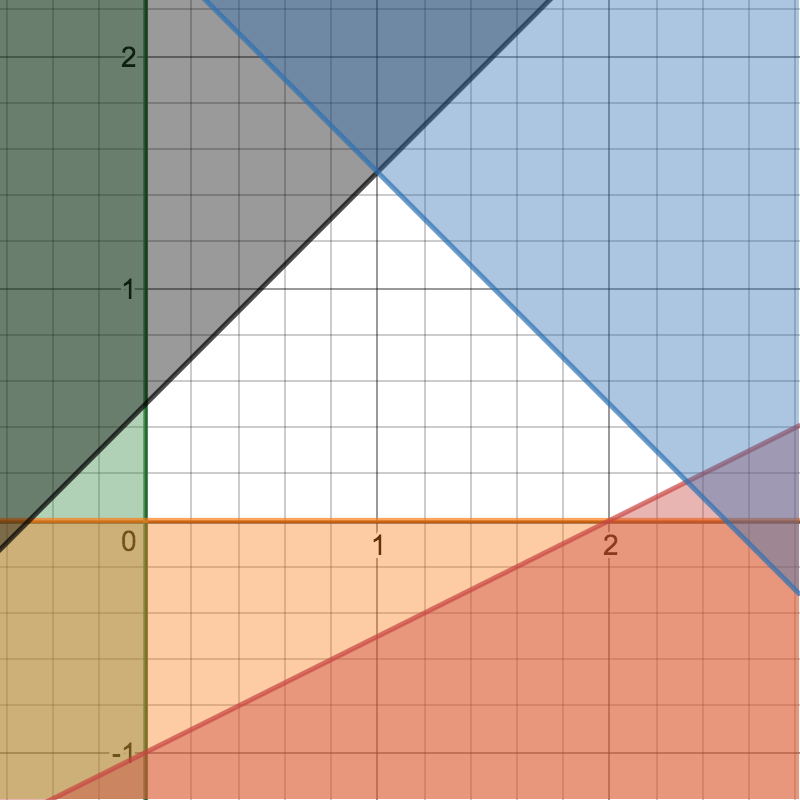
\includegraphics[width=0.9\textwidth]{2014_09_16}
    \caption{Regione di ammissibilità del problema}
  \end{subfigure}
  \caption{Vertice ottimo del problema di minimo}
\end{figure}

\subsubsection*{Riporto variabili}
\begin{align*}
  z = 2, \quad
  x_1 = 1, \quad
  x_2 = \frac{3}{2}, \quad
  s_1 = 0, \quad
  s_2 = 4, \quad
  s_3 = 0
\end{align*}
\subsubsection*{Analisi di sensitività}

\begin{figure}
  \begin{subfigure}{0.49\textwidth}
    \[
      -(1) + \rnd{\frac{3}{2}}c_2 = 0 + \frac{1}{2}c_2 \Rightarrow c_2 = 1
    \]
  \end{subfigure}
  \begin{subfigure}{0.49\textwidth}
    \dddgraph{x_1}{x_2}{0}{3}{0}{1.5}{-3}{-2*x + 2*y  <= 1 &&    +x - 2*y   <= 2 &&    2*x + 2*y   <= 5}{-x+y}
    \caption{$c_2 = 1$}
  \end{subfigure}
  \caption{Analisi di sensitività}
\end{figure}

\subsubsection*{Costruisco problema duale}
\begin{align*}
  \min z_D = y_1 + 2y_2 + 5y_3 \\
  -2y_1 + y_2 + 2y_3 & \geq -1 \\
  2y_1 -2y_2 + 2y_3  & \geq 2  \\
  y_1, y_2, y_3      & \geq 0
\end{align*}
\subsubsection*{Scarti complementari}
\[
  \begin{cases}
    x_1(-2y_1 + y_2 + 2y_3  +1) = 0 \\
    x_2(2y_1 -2y_2 + 2y_3  -2 ) = 0 \\
    y_1(-2x_1 + 2x_2 -1) = 0        \\
    y_2(+x_1 - 2x_2  -2) = 0        \\
    y_3(2x_1 + 2x_2  -5) = 0        \\
  \end{cases}
  \Rightarrow
  \begin{cases}
    -2y_1 + y_2 + 2y_3  +1 = 0 \\
    2y_1 -2y_2 + 2y_3  -2  = 0 \\
    y_2 = 0                    \\
  \end{cases}
  \Rightarrow
  \begin{cases}
    y_1 = \frac{3}{4} \\
    y_3 = \frac{1}{4} \\
    y_2 = 0           \\
  \end{cases}
\]
La soluzione ottima del problema duale corrisponde a quella del primale: $z = z_D = \frac{8}{2} = 2$.
\end{document}